%%%%%%%%%%%%%%%%%%%%% chapter.tex %%%%%%%%%%%%%%%%%%%%%%%%%%%%%%%%%
%
% sample chapter
%
% Use this file as a template for your own input.
%
%%%%%%%%%%%%%%%%%%%%%%%% Springer-Verlag %%%%%%%%%%%%%%%%%%%%%%%%%%
%\motto{Use the template \emph{chapter.tex} to style the various elements of your chapter content.}
\chapter{Attacker Privilege Escalation to Domain Administrator in Active Directory}
\label{intro} % Always give a unique label
% use \chaptermark{}
% to alter or adjust the chapter heading in the running head

\abstract*{Each chapter should be preceded by an abstract (no more than 200 words) that summarizes the content. The abstract will appear \textit{online} at \url{www.SpringerLink.com} and be available with unrestricted access. This allows unregistered users to read the abstract as a teaser for the complete chapter.
Please use the 'starred' version of the new \texttt{abstract} command for typesetting the text of the online abstracts (cf. source file of this chapter template \texttt{abstract}) and include them with the source files of your manuscript. Use the plain \texttt{abstract} command if the abstract is also to appear in the printed version of the book.}


\section{Attacker Privilege Escalation to Domain Administrator in Active Directory}

\subsection{Section 1: Domain Admin Breach}
An attacker’s acquisition of Domain Administrator privileges within an Active Directory (AD) environment represents a critical objective for Advanced Persistent Threats (APTs) and sophisticated nation-state adversaries. This section delineates prevalent methodologies employed to achieve privilege escalation, operating under the \textit{\textbf{assumption of breach}}, wherein the attacker has already established a toehold on an internal system and compromised some domain user or service account via some post-exploitation method.

A stark reality for many enterprise security postures is the often-expedited timeline from initial domain user compromise to full Domain Administrator control. This rapid escalation frequently prompts the critical defensive inquiry: \textit{“How does this occur?”}

The typical attack lifecycle often initiates with targeted reconnaissance, such as targeted spearphishing campaigns or exploitation of vulnerabilities in public-facing web applications, enabling initial arbitrary code executions within the targeted network perimeter. Upon establishing this initial presence, the immediate subsequent phase involves extensive passive or active internal reconnaissance. This recon aims to identify critical assets, discover vulnerabilities and weak entry points into the core network, and mapping or blueprinting of network topology to facilitate the attacker’s efforts for achieving privilege escalation, establishing long-term persistence, and ultimately enabling data exfiltration, often targeting an organization’s most sensitive information assets, or \textit{“crown jewels.”}

While the granular execution details may vary, the overarching progression of such an attack adheres to a consistent thematic flow:

\textbf{1. Initial Access (Malware Injection): }This often involves attack vectors such as spearphishing, impersonation, web exploits, or supply chain compromise.

\textbf{2. Internal Reconnaissance: }Post-compromise, an attacker’s next step after recon is to enumerate network resources, user accounts, group memberships, and potential misconfigurations.

\textbf{3. Credential Theft: }Harvesting of credentials through various cracking techniques, including memory scraping, hash dumping, or keylogging.

\textbf{4. Exploitation and Privilege Escalation: }Leveraging identified vulnerabilities or misconfigurations to elevate access rights, culminating in Domain Admin account breach and compromise.

\textbf{5. Data Access and Exfiltration: }Accessing and extracting targeted sensitive information.

\textbf{6. Persistence: }Establishing mechanisms to maintain long-term access to the compromised environment, even after system reboots, system reimages, or credential changes.

This section commences with the attacker having successfully achieved an internal system toehold, recognizing that this initial breach is often less challenging in contemporary, complex network infrastructures, such as ICS/SCADA networks and critical infrastructure. Furthermore, escalating privileges from a standard workstation user to a \textbf{local administrator} is frequently a straightforward process. This local privilege escalation can manifest through the exploitation of unpatched operating system vulnerabilities or, more commonly, by discovering cached administrative credentials within \textit{Group Policy Preferences (GPPs)} stored in the \texttt{SYSVOL} share.

\subsection{\textbf{1. Passwords in SYSVOL \& Group Policy Preferences (GPPs)}}
This attack vector represents one of the most straightforward methods for an attacker to escalate their privileges within an Active Directory (AD) environment, and often one that requires minimal specialized tooling to accomplish. This attack capitalizes on a historical vulnerability and common misconfigurations within ADs \textit{Group Policy Objects (GPOs).}

\subsubsection{\textbf{Understanding the Vulnerability}}
The \texttt{SYSVOL} share is a domain-wide \textit{Distributed File System (DFS) }share within Active Directory, critical for domain operations. It hosts essential data such as logon scripts, Group Policy data, and other domain-wide information that requires replication across all Domain Controllers (DCs). Crucially, all authenticated users within the domain possess \textbf{read access} to the \texttt{SYSVOL} share, located at \texttt{<DOMAIN>\textbackslash{}SYSVOL\textbackslash{}<DOMAIN>\textbackslash{}Policies\textbackslash{}}.

Prior to 2012, when Group Policy Preferences (GPPs) were introduced, Microsoft implemented a feature allowing administrators to embed credentials (e.g., for creating local users, scheduling tasks, or configuring services) directly within GPP XML files. These passwords were encrypted using \textbf{AES-256}; however, a severe oversight occurred: Microsoft publicly released the \textbf{AES encryption key (shared secret)} on MSDN.

Consequently, any authenticated domain user can enumerate the \texttt{SYSVOL} share, specifically searching for XML files associated with GPPs. The most commonly targeted files include:

\begin{itemize}
    \item \texttt{groups.xml} (for Local Users and Groups GPPs)
    \item \texttt{scheduledtasks.xml} (for Scheduled Tasks GPPs)
    \item \texttt{services.xml} (for Services GPPs)
\end{itemize}

These XML files often contain a field named \textbf{“\texttt{cpassword},”} which holds the AES-256 encrypted password.

\textbf{Important to Note:}
\textbf{AES-256} refers to the \textit{\textbf{Advanced Encryption Standard (AES)}} algorithm using a \textbf{256-bit key length. }It is a highly secure and widely adopted \textit{\textbf{symmetric block cipher}} used globally, including the United States Federal Government, for protecting sensitive digital data at rest or in transit.

\subsection{\textbf{What Is AES?}}

AES is a \textit{symmetric block cipher}, meaning it uses the \textit{same secret key} for both encrypting plaintext (human-readable data) into ciphertext (encrypted, machine-readable data, binary, \texttt{1s} and \texttt{0s}), and decrypting ciphertext back into plaintext. It operates on fixed-size blocks of data, specifically \textbf{128-bit blocks} (16 bytes), regardless of the key size.

The algorithm was established by the U.S. National Institute of Standards and Technology (NIST) in 2001, replacing the older \textit{Data Encryption Standard (DES)} due to DESs shorter key length and susceptibility to brute-force attacks.

\subsubsection{\textbf{Why 256?}}
The “256” in AES-256 indicates the \textbf{length of the cryptographic key} used in the encryption and decryption process. AES supports three primary key lengths: 128-bit, 192-bit, and 256-bit. A longer key length directly translates to a significantly higher number of possible keys, making brute-force attacks (trying to guess and use every possible key until the correct one is found) exponentially more difficult.

For AES-256, there are 2\textsuperscript{256} possible combinations for the key. To put this into perspective, cracking AES-256 through brute-force with current computing technology is considered computationally infeasible, even for the most powerful supercomputers, taking billions of years, literally. It’s often referred to as “military-grade” encryption because it is approved by the U.S. government for securing classified information, including data up to the "\texttt{TOP SECRET"} level.

\subsection{\textbf{How AES-256 Works}}

The AES algorithm operates through a series of complex mathematical transformations performed over multiple \textbf{rounds. }The number of rounds depends on the key length:

\begin{itemize}
    \item \textbf{\textbf{AES-128: }10 rounds}
    \item \textbf{\textbf{AES-291: }12 rounds}
    \item \textbf{\textbf{AES-256: 14 rounds}}
\end{itemize}

Each round consists of a sequence of four fundamental operations applied to the 128-bit data block, represented as a 4 x 4 matrix of bytes:

\textbf{1. \texttt{SubBytes} (Byte Substitution): }Each byte in the data block is replaced with another byte using a predefined substitution box (S-box). This introduces \textbf{non-linearity, }a crucial property for cryptographic strength.

\textbf{2. ShiftRows (Row Shifting): }The rows of the data matrix are cyclically shifted to the left by different offsets. This step provides \textbf{diffusion} by spreading the byte values across the entire block.

\textbf{3. MixColumns (Column Mixing): }A mathematical operation (matrix multiplication) is performed on each column of the data matrix, further scrambling the data and enhancing diffusion. This step is skipped in the final round.

\textbf{4. AddRoundKey (Key Mixing): }A \textbf{round key}, derived from the original 256-bit secret key through a process called \textit{\textbf{key expansion}} is combined with the current data block using a bitwise XOR operation. This step directly integrates the secret key material into the encryption process.

These operations are performed repeatedly for the specified number of rounds. The final round omits the MixColumns step and concludes with an AddRoundKey operation, producing the final ciphertext.

\subsubsection{\textbf{Key Features \& Applications}}

\begin{itemize}
    \item \textbf{\textbf{Symmetric Key Algorithm: }Uses the same key for encryption and decryption (goes both ways). This makes it efficient for encrypting large volumes of data.}
    \item \textbf{\textbf{Block Cipher: }Processes data in fixed-sized blocks of 128-bits.}
    \item \textbf{\textbf{High Security: }Considered virtually unbreakable by brute-force attacks with current technology, offering durable protection against unauthorized access.}
    \item \textbf{\textbf{Substitution-Permutation Network (SPN): }The underlying structure of the algorithm, involving alternating layers of substitutions and permutations to create strong cryptographic mixing.}
    \item \textbf{\textbf{Widely Adopted: }AES-256 is the standard for securing data in various applications, including:}
\end{itemize}

\begin{itemize}
    \item \textbf{\textbf{Data at Rest (DAR): }Full Disk Encryption (FDE) (e.g., BitLocker, FileVault) and database encryption.}
    \item \textbf{\textbf{Data in Transit (DIT): }Secure communication protocols like TLS/SSL (HTTPS), VPNs, and wireless security (WPA2/3).}
    \item \textbf{\textbf{File Encryption: }For sensitive documents and archives.}
\end{itemize}

While AES-256 is highly secure, its effectiveness ultimately depends on proper implementation and the \textbf{secrecy of the key. }A strong algorithm cannot compensate for weak key management practices.

\textbf{Mitigation}

Mitigating the risk of attackers leveraging exposed credentials within SYSVOL and Group Policy Preferences (GPPs) is crucial for preventing
\begin{figure}[htbp]
    \centering
    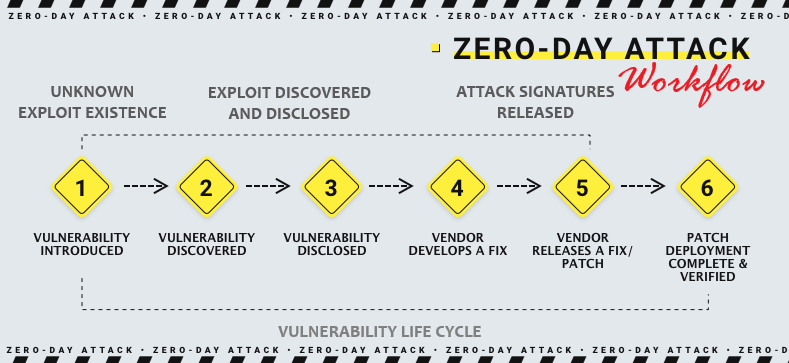
\includegraphics[width=\linewidth]{image.png}
    \caption{Enter Caption}
    \label{fig:image}
\end{figure}

